\section{Software architecture}

\begin{figure}
  \centering
  \makebox[\textwidth][c]{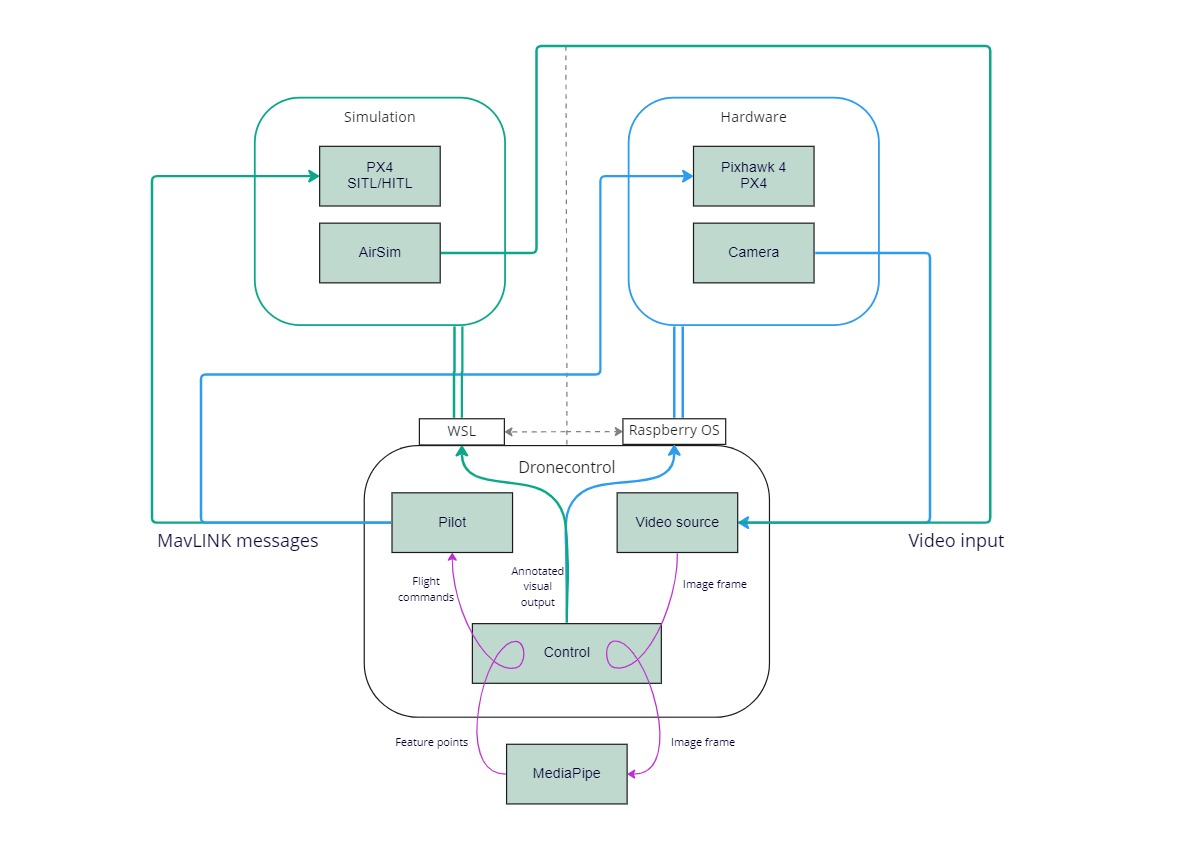
\includegraphics[width=1.2\textwidth, keepaspectratio]{img/software-arch.jpg}}
  \caption{Structure of the DroneVisionControl application and its interactions with the necessary additional software for running in a simulation (green) or a vehicle (blue).}
\label{fig:architecture}
\end{figure}

In this section, the architecture of the designed DroneVisionControl application is presented.
Figure \ref{fig:architecture} illustrates the main modules of the designed software and their interactions with external libraries. The application comprises three fundamental parts: the \textbf{pilot module}, responsible for sending instructions to the flight controller and receiving position and state information through the  \texttt{mavsdk} library; the \textbf{video source module}, which handles image retrieval from various sources and performs necessary image analysis processing; and the \textbf{control module}, which facilitates interaction between the other two modules to convert pixel information into position points using the \texttt{mediapipe} library, and further into instructions for the pilot.

In the upper part of the diagram in Figure \ref{fig:architecture}, the flow of information between the DroneVisionControl application and the external systems is depicted. Green lines represent the path in a simulated workflow, while blue lines indicate the alternative path for a system with actual quadcopter hardware. Purple arrows indicate the input/output of each module within the developed application and how they interconnect. Additionally, smaller utilities have been developed to test the interaction between systems and calibrate different aspects of the control behaviour. These utilities are described in sections \ref{subsec:cam-tool} and \ref{subsec:pid-tools}. A user manual with all the options available in the application can be found in Appendix \ref{app:cli}.

\subsection{Pilot module}
\label{subsec:pilot-module}

The pilot module\footnote{\url{https://github.com/l-gonz/tfg-giaa-dronecontrol/blob/main/dronecontrol/common/pilot.py}} serves the purpose of providing access to the rest of the application for sending and receiving messages from the PX4 controller through the MavSDK library. This library offers a simple asynchronous API for managing one or more vehicles, allowing programmatic access to vehicle information, telemetry, and control over missions, movements, and other operations. The integration of MavSDK with the pilot module utilizes the Python library \texttt{asyncio} \cite{asyncio}, which enables running coroutines in parallel while waiting for messages provided through MAVLink communication.

To interact with the MavSDK library, all calls need to be written as async functions that await the result of one or more polls to the flight stack. The \texttt{asyncio} library provides support for writing concurrent code using the \texttt{async/await} syntax, serving as a foundation for various Python asynchronous frameworks used for high-performance network and web servers, database connection libraries, and distributed task queues. It offers a set of high-level APIs to run Python coroutines concurrently and grants complete control over their execution.

The pilot module, integrating MavSDK and \texttt{asyncio}, provides functionality to establish a connection to a PX4 vehicle through a physical serial address or a UDP endpoint.
During this connection phase, the module will poll for internal information from the flight controller to decide when the system is ready to receive instructions.
The MAVSDK library exposes telemetry and other state information through asynchronous generators, which are defined in Python as a convenient way to retrieve data asynchronously. These are accessed with the \texttt{async\ for} syntax.

The second task of the pilot module is to provide a queue for the control module to send actions to be executed in the vehicle sequentially. It implements many basic operations that can be executed in the flight controller, along with error handling and safety checks. These operations include takeoff, landing, return home, and manipulating the vehicle's flying velocity directly by providing speeds in body coordinates. The actions can be executed directly or added to the queue, which is periodically polled to run the actions in the order they are added. The module ensures that each action waits until the previous one has finished and the vehicle is in the desired state before starting the next action.
It is also designed to allow a maximum time limit of 10 seconds for each action.

To enable direct control of the vehicle's velocity, a special flight mode defined by PX4, called Offboard mode\footnote{\url{https://docs.px4.io/main/en/flight_modes/offboard.html\#offboard-mode}}, is required (not related to the offboard configuration described in Section \ref{subsec:offboard}). Offboard mode primarily controls vehicle movement and attitude, adhering to setpoints provided through MAVSDK. This mode relies on position or pose/attitude information available to the flight controller, such as through a gyroscope and a GPS antenna. 
For safety purposes, this mode requires a constant stream of commands to be maintained.
If the message rate falls below 2Hz or the connection is lost, the vehicle will come to a halt and, after a timeout, attempt to land or perform other failsafe actions based on the configured parameters.
This behaviour is handled internally by the MAVSDK library and made available to the application by the pilot module through a \texttt{toggle\_offboard\_mode} function.

By encapsulating the functionality of sending commands and receiving information from the flight controller, the pilot module provides a robust interface for controlling the vehicle's behaviour and enables seamless integration with other components of the application.


\subsection{Video source module}
\label{subsec:viz-source-module}

The video source module\footnote{\url{https://github.com/l-gonz/tfg-giaa-dronecontrol/blob/main/dronecontrol/common/video_source.py}} aims to provide a collection of classes to retrieve images from different sources in a manner that allows easy interchangeability without affecting the rest of the application. 
This design facilitates testing and adaptability to various environments. Three classes of video sources have been implemented: file, simulator, and camera, all of which inherit from the \texttt{VideoSource} class, as shown in the diagram in Figure \ref{fig:video-source-inheritance}.

\begin{figure}
  \centering
  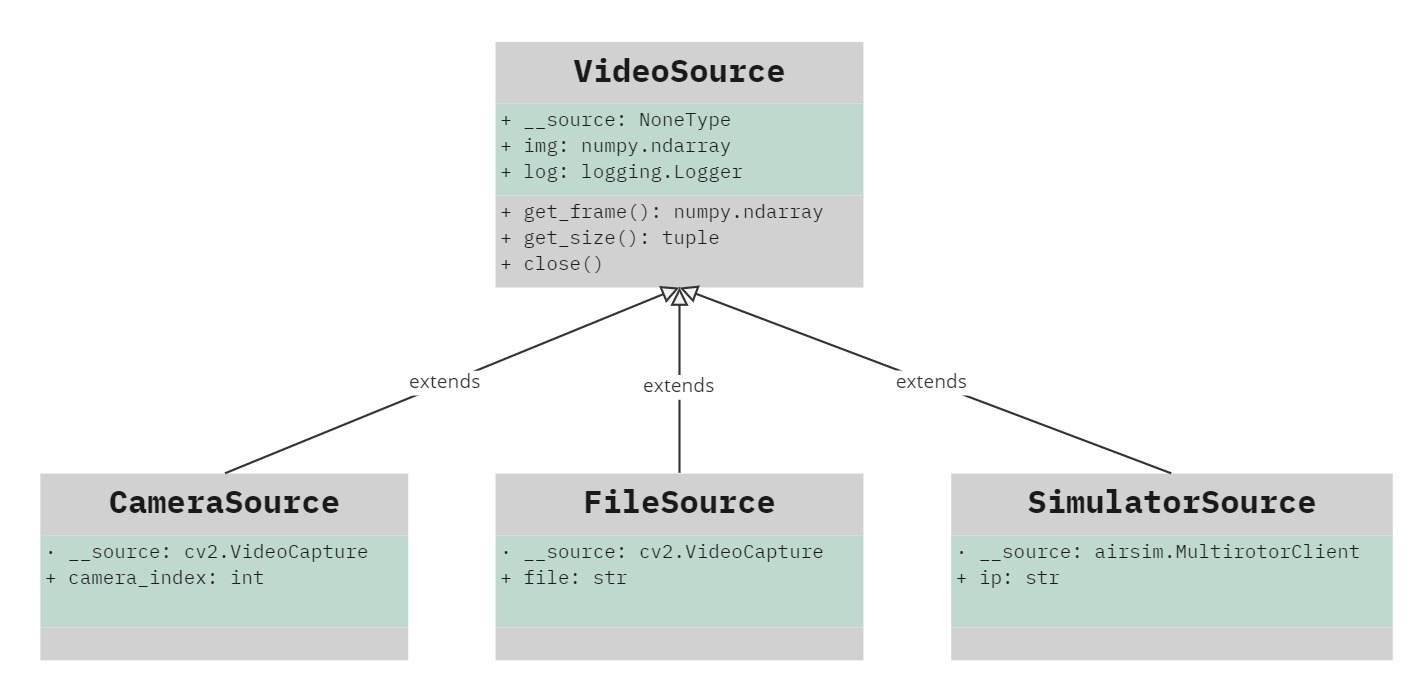
\includegraphics[width=\textwidth, keepaspectratio]{img/uml-video-source.jpg}
  \caption{Diagram of inheritance on the video source classes available to retrieve image data.}
  \label{fig:video-source-inheritance}
\end{figure}

The \texttt{FileSource} class can open a video file stored on the companion computer and provide frames sequentially until the video is completed. This feature enables the replaying image detection algorithms on previously captured videos using the camera tool described in section \ref{subsec:cam-tool}. The \texttt{CameraSource} class can access a physical camera connected to the computer running the application via USB and provide real-time captured frames. Both the file and camera sources leverage OpenCV's video capture utilities to handle file operations and camera drivers.

The \texttt{SimulatorSource} utilizes AirSim's Python library, \texttt{airlib}, to communicate with the simulator and retrieve images from a camera object attached to the vehicle model in Unreal Engine. It establishes an automatic connection to the simulator via \texttt{localhost}, but it can also be initialized with an IP address to connect to a simulator running on a different computer within the local network. This is particularly useful when the DroneVisionControl runs inside a Linux subsystem (WSL) and the simulator operates on the host Windows system.

\subsection{Vision control module}
\label{subsec:control-module}

The control module encompasses the main logic of the application and is responsible for converting raw images obtained from the video source into commands for the pilot module. Two different types of control solutions have been implemented. The first one is the proof-of-concept control solution described in Section \ref{sec:hands}, operating in the offboard configuration outlined in Section \ref{subsec:offboard}. Its purpose is to translate predefined hand gestures into movement commands for the aerial vehicle. This solution facilitates testing the interaction between all system components in a contained environment by situating the controlling computer outside of the vehicle. The second control system is a follow mechanism, described in Section \ref{sec:follow}, which aims to mimic real-life scenarios where the control algorithms and camera reside onboard the vehicle. It tracks the location of a person detected in the images captured from the drone's perspective and uses that information to calculate velocities necessary for following and keeping the person centred in the drone's view.

Both solutions follow a similar process. Initially, the image is sent to the MediaPipe computer-vision third-party library, described in Section \ref{subsec:mediapipe}, which extracts the required features from the image in the form of 2D coordinates. Subsequently, various calculations specific to each solution are applied to these coordinates to determine the commands sent to the pilot module.
Captured images, detected features and calculated results are communicated to a simple \acrshort{gui}, drawn with the help of the OpenCV library. This interface shows the user all the necessary information about the current state of the running application.

Sections \ref{sec:hands} and \ref{sec:follow} provide further explanations of the control modules used in the two different solutions developed.

\subsection{Camera-testing tool}
\label{subsec:cam-tool}

In addition to the main modules, several utilities have been included in the DroneVisionControl program to facilitate the development and testing processes of the control solutions. The first tool is available in the \texttt{test\_camera} module\footnote{\url{https://github.com/l-gonz/tfg-giaa-dronecontrol/blob/main/dronecontrol/tools/test_camera.py}} and can be accessed through the command \texttt{dronevisioncontrol tools test-camera}. This tool serves multiple purposes, including testing the connection between the computer, the flight stack, and the camera without needing to attach any self-guided control mechanism. It also allows evaluation of the performance of the MediaPipe hand and pose machine learning solutions on real-time images. Additionally, it enables image capture and video recording from a live camera feed for subsequent analysis. 

The test tool can be configured through command-line options to use any of the three available video sources (camera, simulator, or video file), connect to a hardware or simulated PX4 flight controller by specifying a connection string or IP, and run on any system acting as a companion computer. Computer vision can optionally be enabled to process incoming images using hand or pose recognition software. While the tool is running, basic commands such as takeoff, landing, or movement along any direction can be sent to a connected vehicle using the keyboard. Appendix \ref{app:cli} provides a comprehensive breakdown of all the tool's options.


\section{Proof of concept: hand-gesture solution}
\label{sec:hands}
This solution was developed to test that the flow of the application works as expected, both in simulation and in actual flight, and that all the systems can interact and establish the required connections with each other.
For that reason, it is designed to run with as little setup as possible. Flight tests can be undertaken with the minimal hardware components in the offboard configuration (Figure \ref{fig:offboard-config}).

The control module for this solution is the \texttt{mapper} module\footnote{\url{https://github.com/l-gonz/tfg-giaa-dronecontrol/blob/main/dronecontrol/hands/mapper.py}}.
It runs on a loop that continuously polls for a new frame from the chosen video source and feeds it to the hand detection functionality provided by MediaPipe \cite{mp-hands-paper}.
If a hand is detected in the image, 2D coordinates called landmarks are extracted according to the mapping in figure \ref{fig:hand-landmarks}.
These landmarks are then converted into discrete gestures, such as an open palm, closed fist, or finger pointing in different directions. Each detected gesture is assigned a command, which is queued to the pilot module and executed once the previous commands have been completed.

\begin{figure}
  \centering
  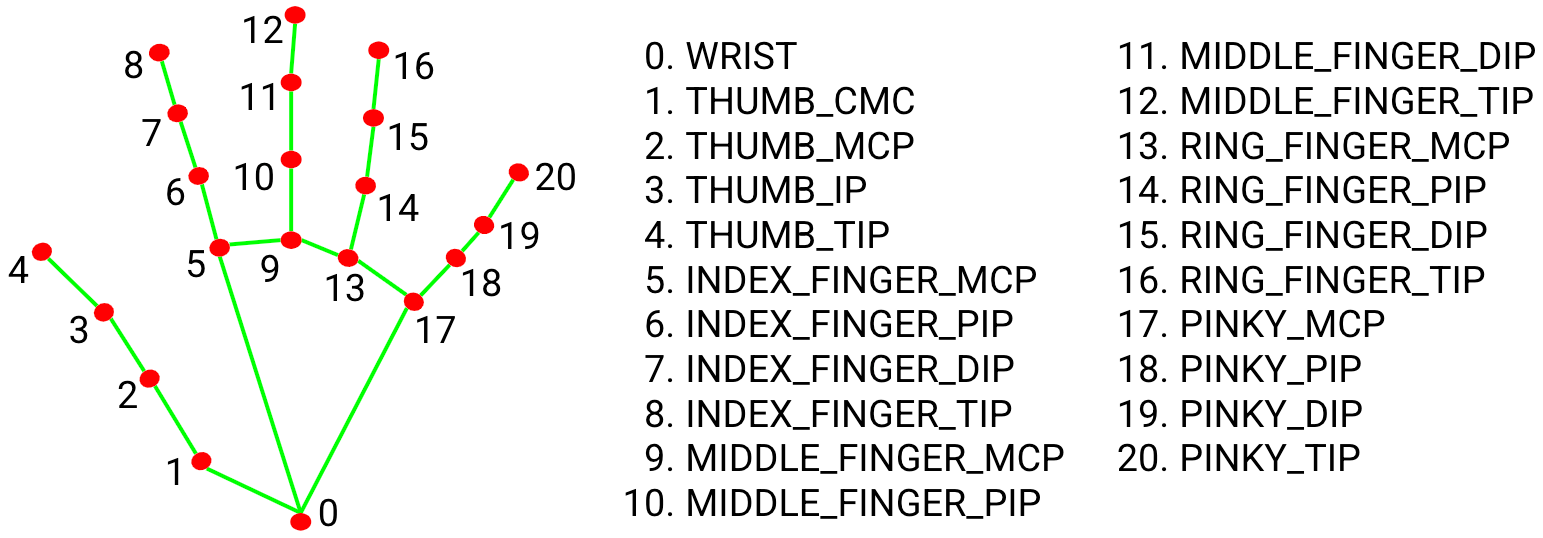
\includegraphics[width=\textwidth, keepaspectratio]{img/hand_landmarks.png}
  \caption{Landmarks extracted from detected hands by the MediaPipe hand solution.}
  \source{Adapted from \citetitle{mp-hands} \cite{mp-hands}.}
  \label{fig:hand-landmarks}
\end{figure}

The conversion from landmarks to gestures is performed by the \texttt{gestures} module\footnote{\url{https://github.com/l-gonz/tfg-giaa-dronecontrol/blob/main/dronecontrol/hands/gestures.py}}. Vectors are drawn from the base of each finger to its tip, as well as from the base of the hand (wrist feature) to the base of the fingers. The dot product vector operation is used to calculate the relative angles between each finger and the base of the hand, as shown in figure \ref{fig:vector-calcs}. By comparing these angles to a threshold, the module can determine whether each finger is extended or folded and in which direction it points. For example, an open hand gesture is detected when all five fingers are extended.

\begin{figure}
  \centering
  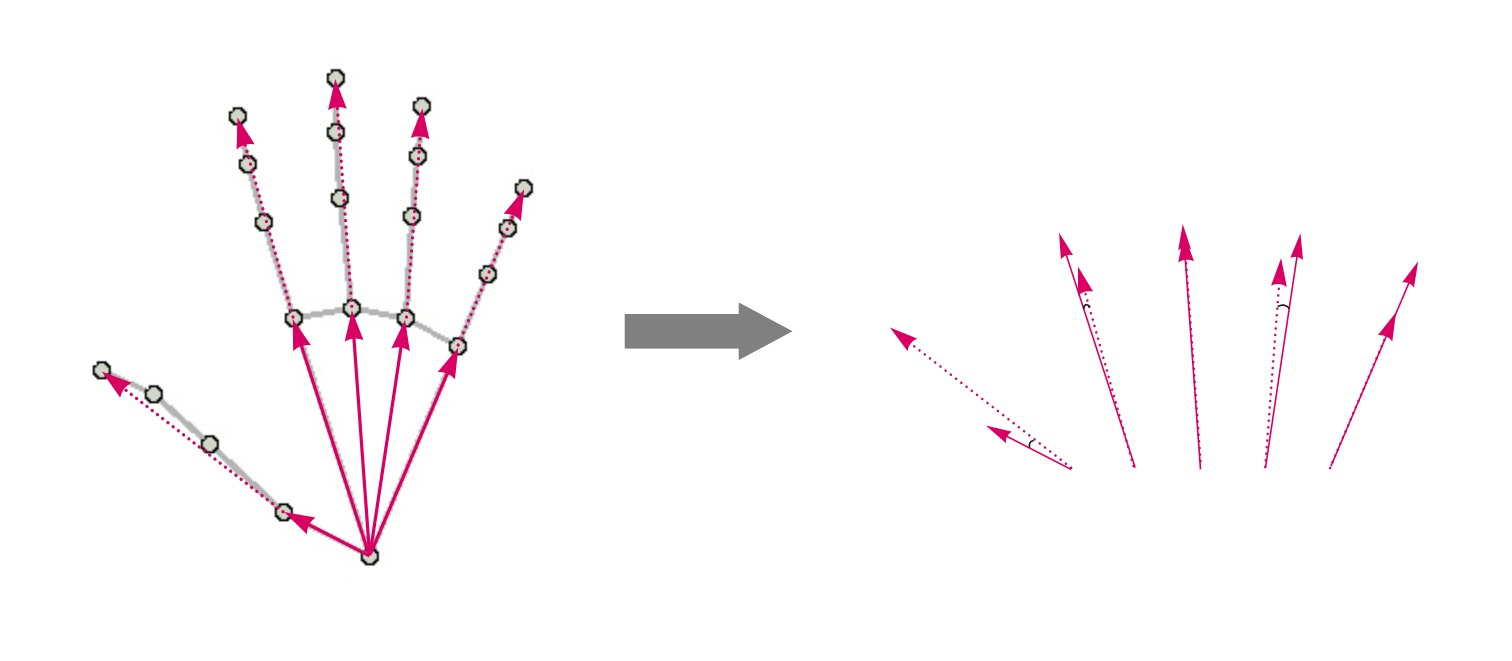
\includegraphics[width=0.9\textwidth, keepaspectratio]{img/hand-vectors.jpg}
  \caption{Vectors extracted from the detected features are used to calculate reference angles to determine hand gestures.}
  \label{fig:vector-calcs}
\end{figure}

The program defines several gestures based on the calculated angles. These gestures are shown in Figure \ref{fig:hand-gestures} and detailed in the following list:
\begin{itemize}
    \item No hand: this happens when no landmarks can be extracted from the image. As a safety feature, the vehicle stops whichever previous commands it had in its queue and goes into Hold flight mode, hovering in the air while maintaining its position.
    \item Open hand: all five fingers extended, indicating a stop gesture. The drone holds at its current position.
    \item Fist: all five fingers folded into a fist. The drone arms and takes off if on the ground, or lands if already in the air.
    \item Backhand: the back of the hand is shown towards the camera, with the thumb pointing upwards and the other fingers pointing to the side. This gesture puts the drone in Return flight mode, where it climbs to a safe altitude and returns to the last takeoff position.
    \item Index finger pointing up: The index finger is extended and pointing roughly towards the top of the image (within $\pm$30 degrees). The drone enters Offboard flight mode, allowing direct velocity commands. The drone remains in this mode as long as the finger is extended, and its movement can be controlled with any of the next four commands.
    \item Index finger pointing to the right: The index finger points to the right of the image (between 30 and 90 degrees from the top). The drone rolls towards its right side at a speed of 1 m/s.
    \item Index finger pointing to the left: Same as above, but the index finger points to the left of the image. The drone rolls towards its left side.
    \item Thumb pointing to the right: The index finger is extended up (to maintain Offboard flight mode) while the thumb is folded over the palm, pointing towards the right of the screen. This gesture makes the drone pitch forward at a steady speed of 1 m/s.
    \item Thumb pointing to the left: Similar to the previous gesture, but the drone pitches backwards when the thumb points to the left of the screen.
\end{itemize}

\begin{figure}
  \centering
  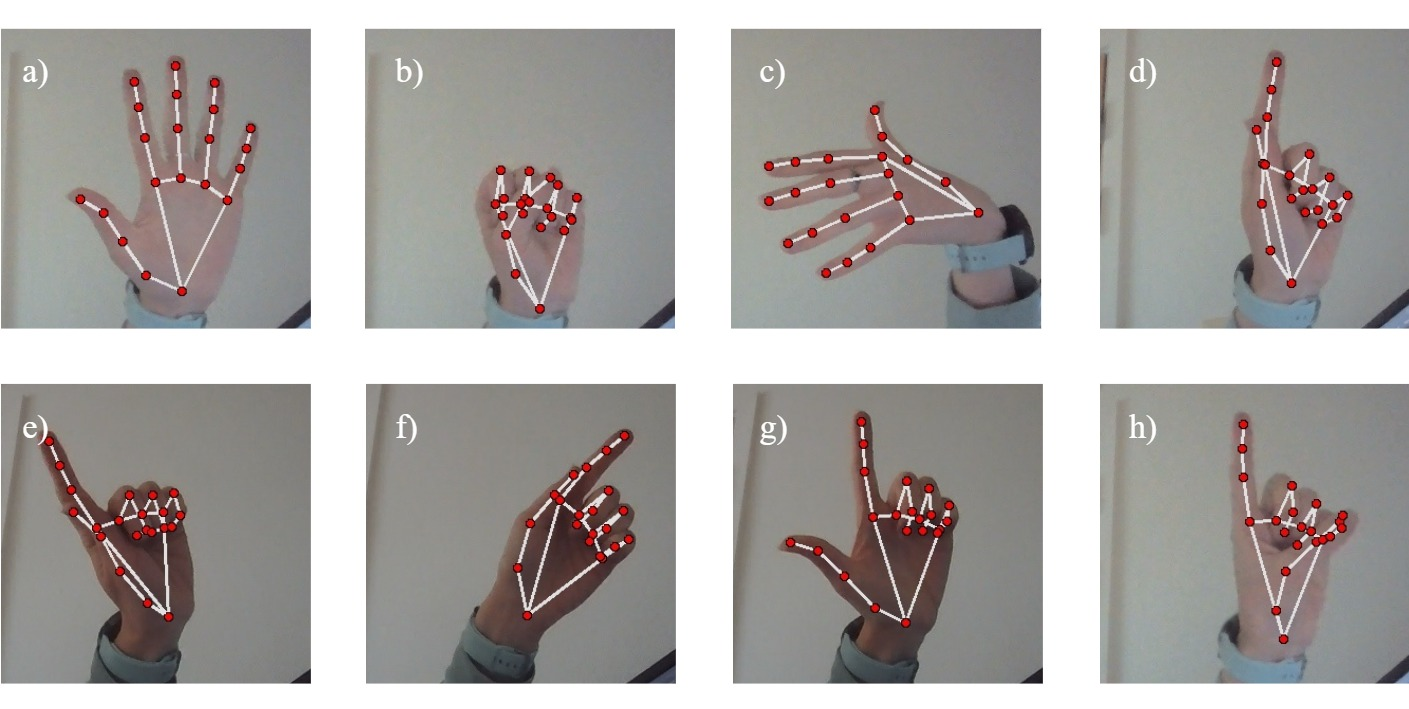
\includegraphics[width=\textwidth, keepaspectratio]{img/hand-gestures.jpg}
  \caption{Gestures detected by the program to control the drone's movement. a) Open hand, b) fist, c) backhand, d) index point up, e) index point left, f) index point right, g) thumb point left, h) thumb point right}
  \label{fig:hand-gestures}
\end{figure}


The program execution is outlined in figure \ref{fig:hands-loop}.
After all the initial parameters have been set, a secondary thread is started to run the pilot queue detailed in \ref{subsec:pilot-module}, which waits for new commands to be added.
The main thread runs a GUI loop that continuously processes gestures calculated from retrieved images and generates actions that are queued for the pilot.
It also recognizes user input on the keyboard to control the vehicle directly, according to the mapping defined in the \texttt{input} module\footnote{\url{https://github.com/l-gonz/tfg-giaa-dronecontrol/blob/main/dronecontrol/common/input.py}}.
\todo[inline]{Link here wherever the mapping is detailed (Appendix?)}

\begin{figure}
  \centering
  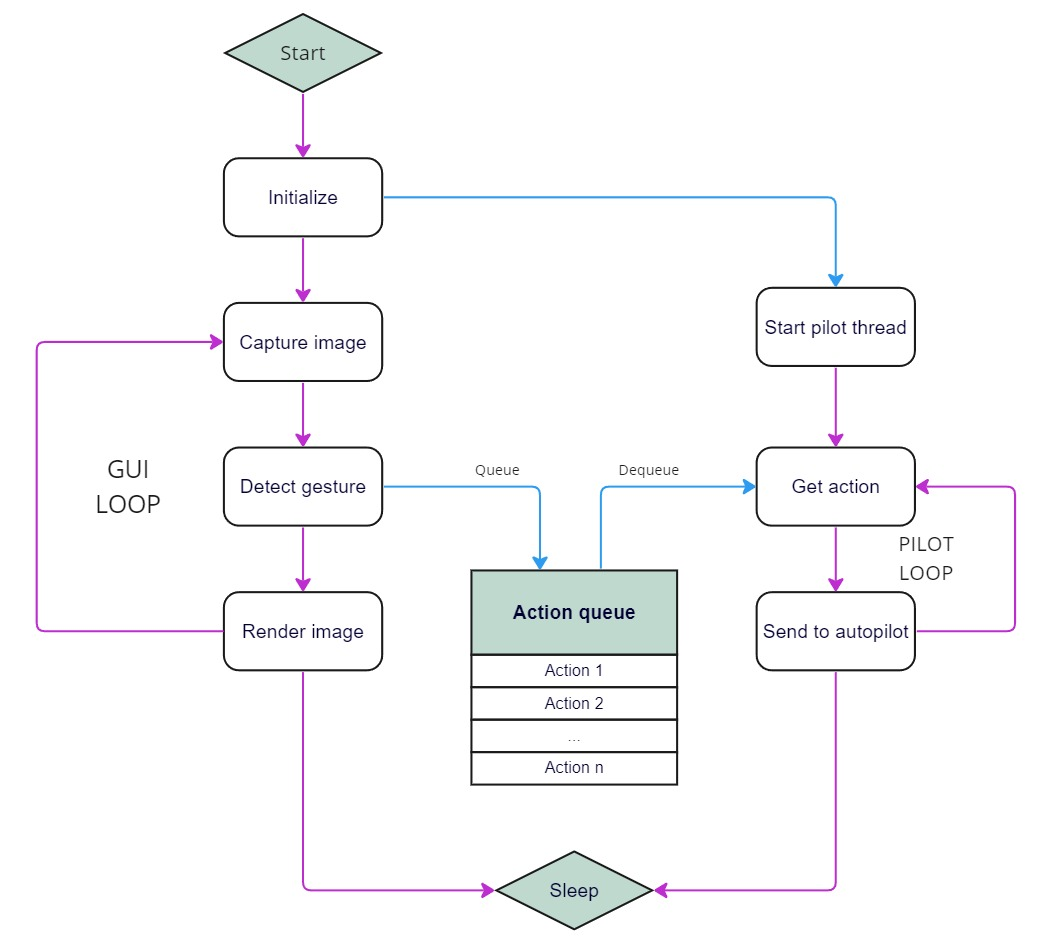
\includegraphics[width=0.8\textwidth, keepaspectratio]{img/hand-loop.jpg}
  \caption{Execution flow for the running loop in the hand-gesture control solution.}
  \label{fig:hands-loop}
\end{figure}

A complete run of this solution is detailed in Section \ref{subsec:fl-test-4}.


\section{Final solution: human following}
\label{sec:follow}

The intention behind developing a UAV control solution that implements tracking and following of humans is to demonstrate the capabilities of the PX4 open-source development platform and its related projects, MAVLink and MAVSDK. The goal is to showcase how complex real-life applications can be designed without relying on expensive proprietary hardware. The follow application requires only a PX4-enabled flight controller installed in an aerial vehicle, a companion computer of appropriate dimensions mounted on board the vehicle, and a camera connected to the companion computer via USB.

In this solution, the vehicle will attempt to find a single person in its field of view and follow their movements by changing its yaw and forward velocity to match horizontal movements and distance changes, respectively.
During program execution, the drone can be controlled via an RC controller, an external ground station application or keyboard input directly to the companion computer through, for example, a remote shell (SSH) or a desktop sharing program.

For safety reasons, the follow mechanism only engages when the flight mode on the vehicle is changed to Offboard mode. This can be done by activating a configured switch on the RC controller. The self-guided control automatically stops if the connection to the computer is lost or if any of the configured fail-safes are triggered, such as low battery, loss of RC or GPS signal, or exceeding predefined pitch and roll limits for a specified time.

\begin{figure}
  \centering
  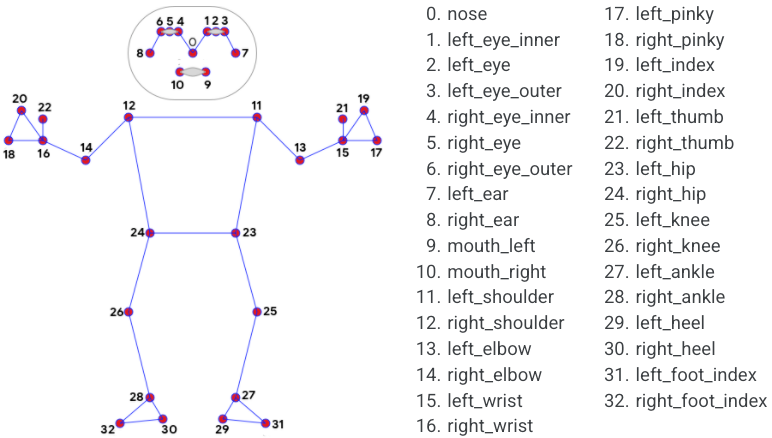
\includegraphics[width=\textwidth, keepaspectratio]{img/pose-landmarks.png}
  \caption{Landmarks extracted from detected human figures by the MediaPipe Pose solution}
  \source{Adapted from \citetitle{mp-pose} \cite{mp-pose}}
  \label{fig:pose-landmarks}
\end{figure}

In offboard mode with the follow mechanism engaged, the system continuously retrieves images from the onboard camera. These images are processed using the MediaPipe Pose \cite{mp-pose-paper} computer vision library to extract pose landmarks in the form of 2D coordinates. 
Figure \ref{fig:pose-landmarks} shows the features extracted by the algorithm and their correspondence to the human body.
The extracted landmarks are used to draw a bounding rectangle around the detected person and validate that the received landmarks match the expected pose of a person standing up.

\begin{figure}
  \centering
  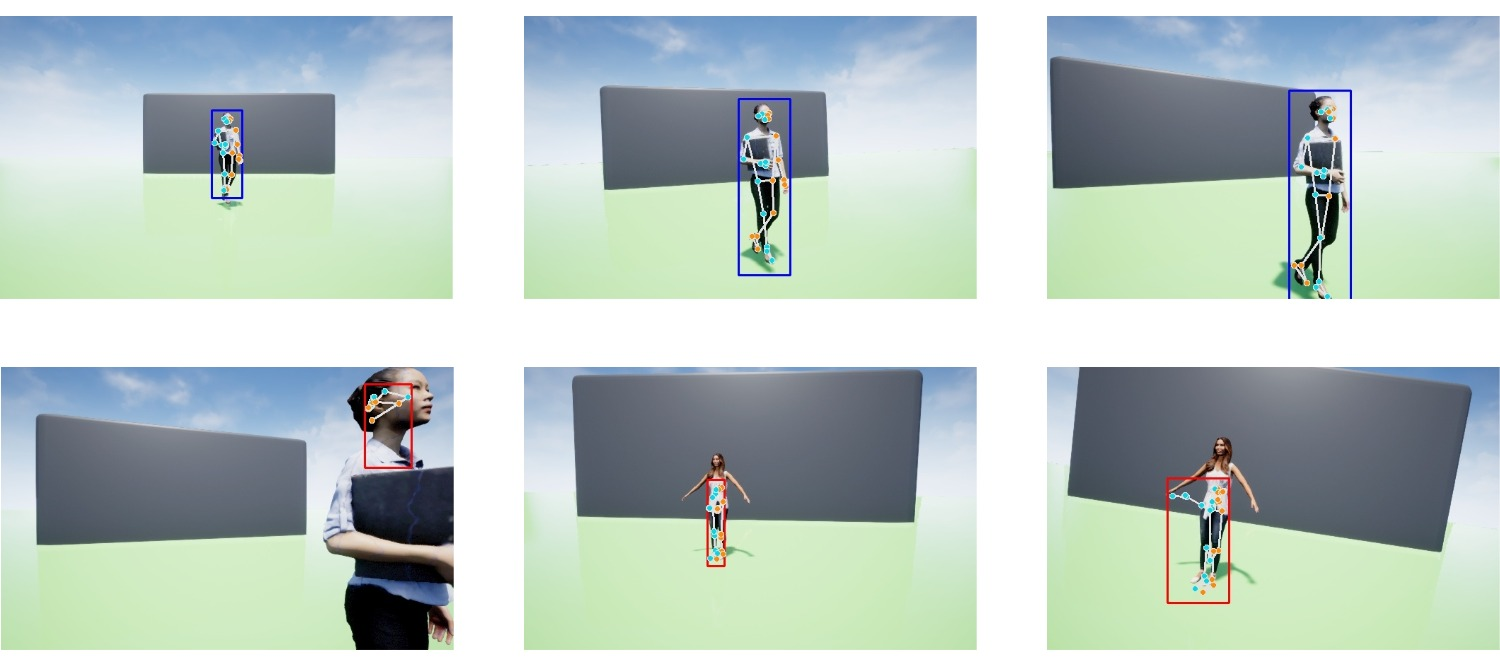
\includegraphics[width=\textwidth, keepaspectratio]{img/pose-validation.jpg}
  \caption{Valid versus invalid poses detected by the follow solution}
  \label{fig:pose-validation}
\end{figure}

Figure \ref{fig:pose-validation} shows some examples of the validation checks running on the raw landmarks extracted from an image.
To ensure controlled movements, the vehicle will stop and hover if it becomes impossible to detect a person in the image or if the detected features do not match the expected pose. Once a valid bounding box is defined around the target person, its position relative to the camera's field of view is sent to a control mechanism consisting of two independent PID controllers. The theory behind these controllers is explained in section \ref{subsec:pid-tools}.

The first PID controller is responsible for controlling the yaw velocity of the vehicle to respond to horizontal movements of the person in the image. It aims to keep the person centred horizontally in the field of view by maintaining the x-coordinate of the bounding box's centre at the middle point of the screen.
The second PID controller controls the forward velocity of the vehicle to respond to changes in the distance between the followed person and the drone. It adjusts the drone's forward movement to keep the height of the bounding box (as a percentage of the total image height) within a desired range. The target height for the controller needs to be set for each video source and desired distance empirically, as it depends on the camera used.
Figure \ref{fig:follow-input-calcs} shows how the inputs for each controller are extracted from the coordinates of the bounding box detected around the figure.

\begin{figure}
  \centering
  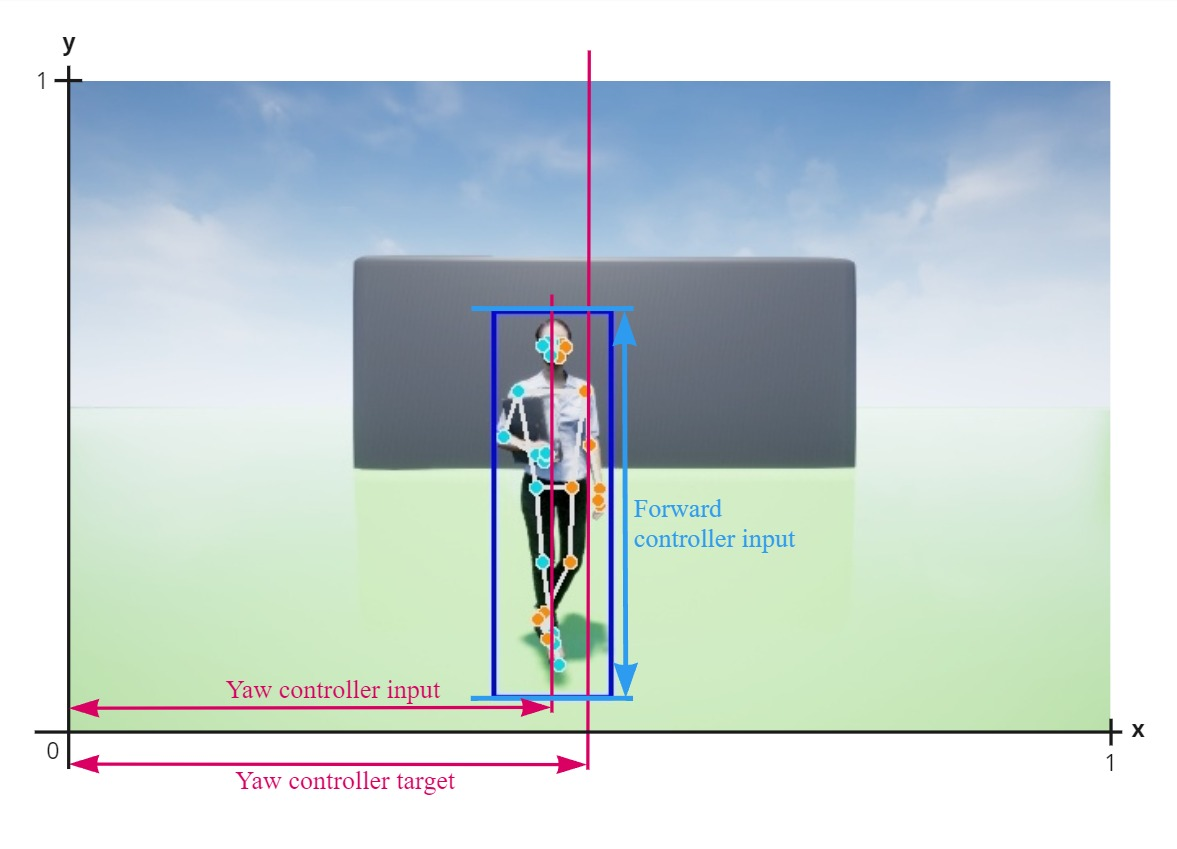
\includegraphics[width=\textwidth, keepaspectratio]{img/pose-calculations.jpg}
  \caption{Calculation of horizontal position and height of figure from the detected bounding box.}
  \label{fig:follow-input-calcs}
\end{figure}

The follow\footnote{\url{https://github.com/l-gonz/tfg-giaa-dronecontrol/blob/main/dronecontrol/follow/follow.py}} module's structure is summarized in a diagram in Figure \ref{fig:follow-loop}.
In each execution, after connecting to the pilot module with the starting options provided, the main loop runs continuously until the user quits the program.
For each iteration, an image is retrieved, pose features are extracted, and a bounding box is calculated. If the vehicle is in Offboard flight mode, the calculated positions are used as inputs for the PID controllers, which generate velocity outputs to be sent to the pilot module. Additionally, manual keyboard control is available to send direct commands to the vehicle.

\begin{figure}
  \centering
  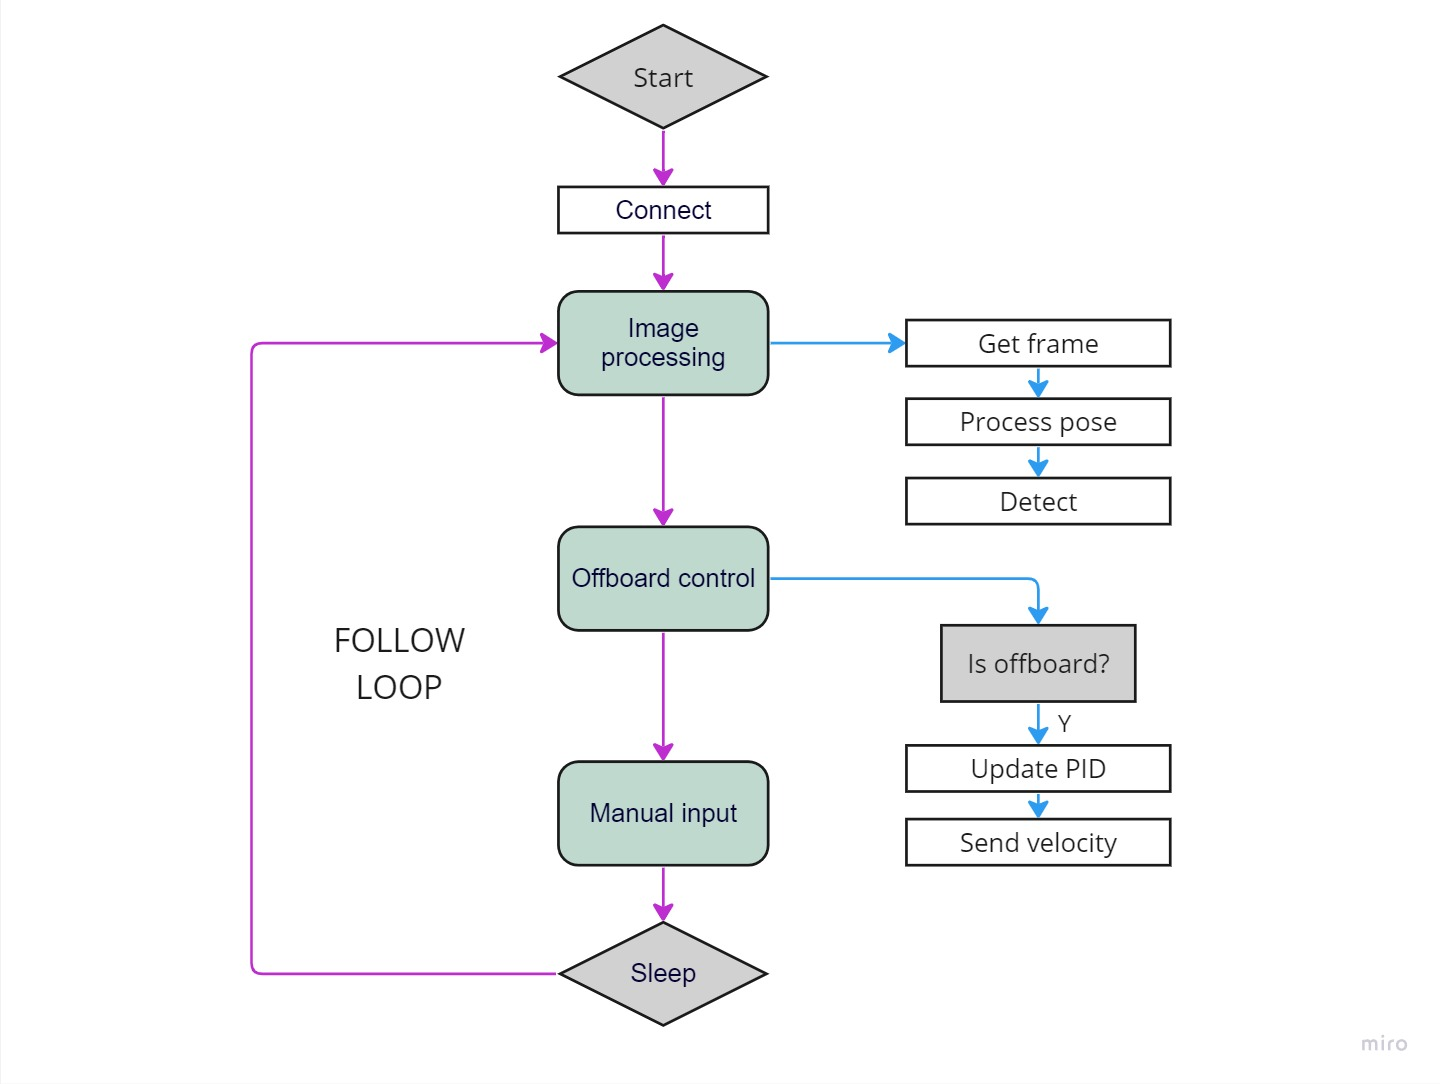
\includegraphics[width=0.9\textwidth, keepaspectratio]{img/follow-loop.jpg}
  \caption{Execution flow for the running loop in the follow control solution}
  \label{fig:follow-loop}
\end{figure}

A full execution of this solution is shown in flight in Section \ref{subsec:fl-test-5}.


\subsection{PID tools}
\label{subsec:pid-tools}

A proportional-integral-derivative (PID) is a control loop mechanism commonly used in systems requiring continuously modulated control. It works by continuously calculating an error value from the difference between the received input on a chosen process variable, which in this case is the detected position of a person in the frame, and the desired set point for that variable, a position centred in the frame. From the error value, the output for the controller is calculated according to this equation:

\begin{equation}
    u(t)= K_p e(t) + K_i \int{e(t)dt} + K_d \frac{de(t)}{dt}
    \label{eq:pid}
\end{equation}
\begin{conditions}
u(t)  &   PID control variable \\
K_p   &   proportional gain \\
K_i   &   integral gain \\
K_d   &   derivative gain \\
e(t)  &   error value \\
de    &   change in error value \\
dt    &   change in time
\end{conditions}

The PID controllers in this project are implemented with the help of the freely-available \texttt{simple-pid} library for Python \cite{pid-library}, which supplies all the necessary calculations.
It is only necessary to provide the coefficients or tunings ($K_p$, $K_i$, $K_d$) and the set point (target value) for the controller at the start and then update it periodically with the current input value to receive the output velocity.
In the DroneVisionControl application, it is the \texttt{controller}\footnote{\url{https://github.com/l-gonz/tfg-giaa-dronecontrol/blob/main/dronecontrol/follow/controller.py}} module the one that interacts with the \texttt{simple-pid} library to feed and receive the correct values to the PID controllers calculated from the bounding box around the detected person.
Two additional utilities have been developed for tuning and testing the performance of the PID controllers.

The first utility is called \texttt{tune\_controller}\footnote{\url{https://github.com/l-gonz/tfg-giaa-dronecontrol/blob/main/dronecontrol/tools/tune_controller.py}}. Tuning a PID controller typically involves testing different combinations of coefficients empirically. The \texttt{tune\_controller} tool facilitates this process by allowing users to specify a range of potential coefficients and testing the system's response using images retrieved from AirSim and a simulated flight controller (SITL or HITL). The tool sets up a simulated person in an offset position from the target centre, engages the controller with the test values, and plots the detected position input and calculated velocity output on a graph for analysis. After each test, the vehicle returns to the starting position to reset the environment for the next coefficient to be checked. The tool can be executed using the command \texttt{dronevisioncontrol tools tune} and can be started with the option \texttt{--yaw} or \texttt{--forward} to tune a specific controller while deactivating the other one for better visualization. Each coefficient can be tested individually by providing fixed values for the other two parameters.

The second utility is called \texttt{test\_controller}\footnote{\url{https://github.com/l-gonz/tfg-giaa-dronecontrol/blob/main/dronecontrol/tools/test_controller.py}}. This tool is designed to evaluate the performance of an already-tuned controller with different position inputs for the camera. The objective is to assess how the controller reacts to varying relative positions between the vehicle and the person being followed. The tool engages both the yaw and forward controllers simultaneously to simulate real flight conditions. However, it can be run in either yaw or forward mode to vary distances in one of the two axes (left to right and forward to backwards, respectively). The tool measures how the vehicle responds to increasingly larger differences from the target position. The purpose is to ensure that the controller maintains a stable movement that ensures safety throughout the entire flight. The test tool's execution and results are detailed in section \ref{subsec:pid-test-controller} of the project documentation.

\subsection{Safety mechanisms}
\label{subsec:safety}

The DroneVisionControl application implements a very experimental vision-based guidance system.
Therefore, to carry out flight tests in real-life conditions, it is necessary to ensure that there are sufficient safety mechanisms to prevent accidents.
These measures include both software-based defences within the application code and safety configurations provided by the PX4 autopilot.

To begin with, the computer vision module in DroneVisionControl verifies the validity of objects detected as a person by examining specific features associated with a standing human figure. It checks that the height of the bounding box is greater than its width and that the features of the head, shoulder, hip, knee, and ankle are detected in the correct order from top to bottom. If any of these checks fail or if no detection output is received, the vehicle immediately enters Hold flight mode. In this mode, any queued velocity commands are discarded, and the drone hovers in its current position. These validation checks are implemented in the \texttt{image\_processing}\footnote{\url{https://github.com/l-gonz/tfg-giaa-dronecontrol/blob/main/dronecontrol/follow/image_processing.py}} module.

In addition to input validation, the application incorporates safety measures related to the PID controllers and the pilot module, which limit the maximum possible velocity of the vehicle at all times during the execution. The PID controllers have output limits set within DroneVisionControl to prevent abnormal velocity commands from being sent to the flight controller. Furthermore, the PX4 autopilot provides a fallback safety measure through its \texttt{MPC\_XY\_VEL\_ALL} parameter, which limits the overall horizontal velocity of the vehicle. These limitations ensure that the drone's movements are within a safe and controllable range.

The PX4 autopilot itself offers various safety configuration options, known as failsafes, documented in \citetitle{px4-docs-safety} \cite{px4-docs-safety}. These failsafes detect undesired conditions during flight and include detecting a lost connection to the companion computer while in Offboard mode, a loss of RC transmitter link or GPS position, low battery levels during flight, and unexpected flipping of the vehicle. When any of these conditions are detected, the autopilot triggers a flight mode change to either Hold (hover) or Return (fly back to takeoff position and land), ensuring the safety of the drone and its surroundings.

The last safety mechanism to mention is not based on automatic detection by the developed software or the autopilot but on active surveillance of the system's behaviour during flight by the operator in control of the vehicle.
With an RC controller configured with a switch to control flight mode, it is possible to deactivate Offboard mode at any moment, which will make the vehicle disregard all instructions from the companion computer and assume complete control of the vehicle either through a GPS-assisted mode or fully manual flight.
A secondary switch in the RC controller can be configured as a kill switch for a last-resort option to stop all motor outputs immediately.
This possibility is most useful when the vehicle is on the ground and cannot manage to take off upwards since there is a danger of breaking the propellers against the ground.

Lastly, operator control plays a vital role in ensuring safety during flight. The operator can use an RC controller with a designated switch to deactivate Offboard mode at any time. This action causes the vehicle to disregard instructions from the companion computer and assume control through GPS-assisted or manual flight modes. Additionally, a secondary switch can be configured as a kill switch, allowing for an immediate stop of all motor outputs when needed. This feature is particularly useful in situations where the vehicle is on the ground and has trouble taking off to reduce the risk of propeller damage if the vehicle flips.

By integrating these safety mechanisms, the DroneVisionControl application aims to mitigate potential risks and ensure safe flight operations under real-life conditions.